
% \begin{figure}[t]
%   \centering
  
%   \begin{minipage}[t]{0.504\textwidth}
%   \centering
%   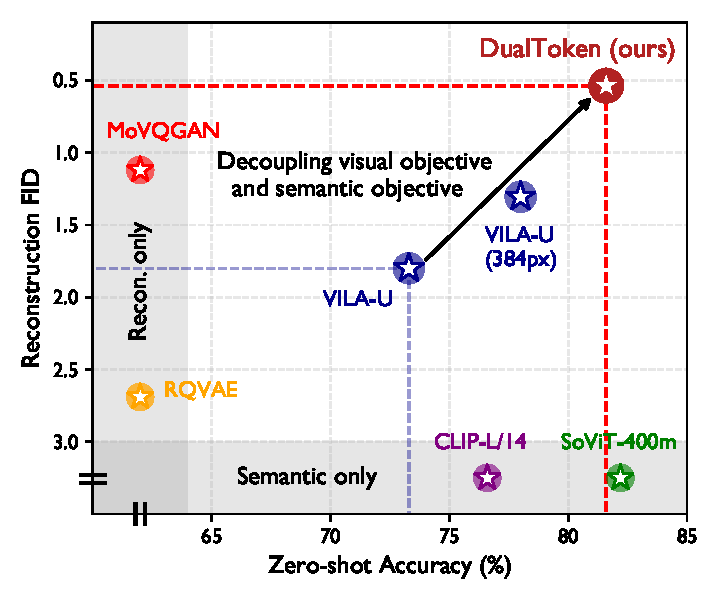
\includegraphics[height=5.2cm]{imgs/bubble.pdf}
%   \end{minipage}
%   \begin{minipage}[t]{0.44\textwidth}
%   \centering
%   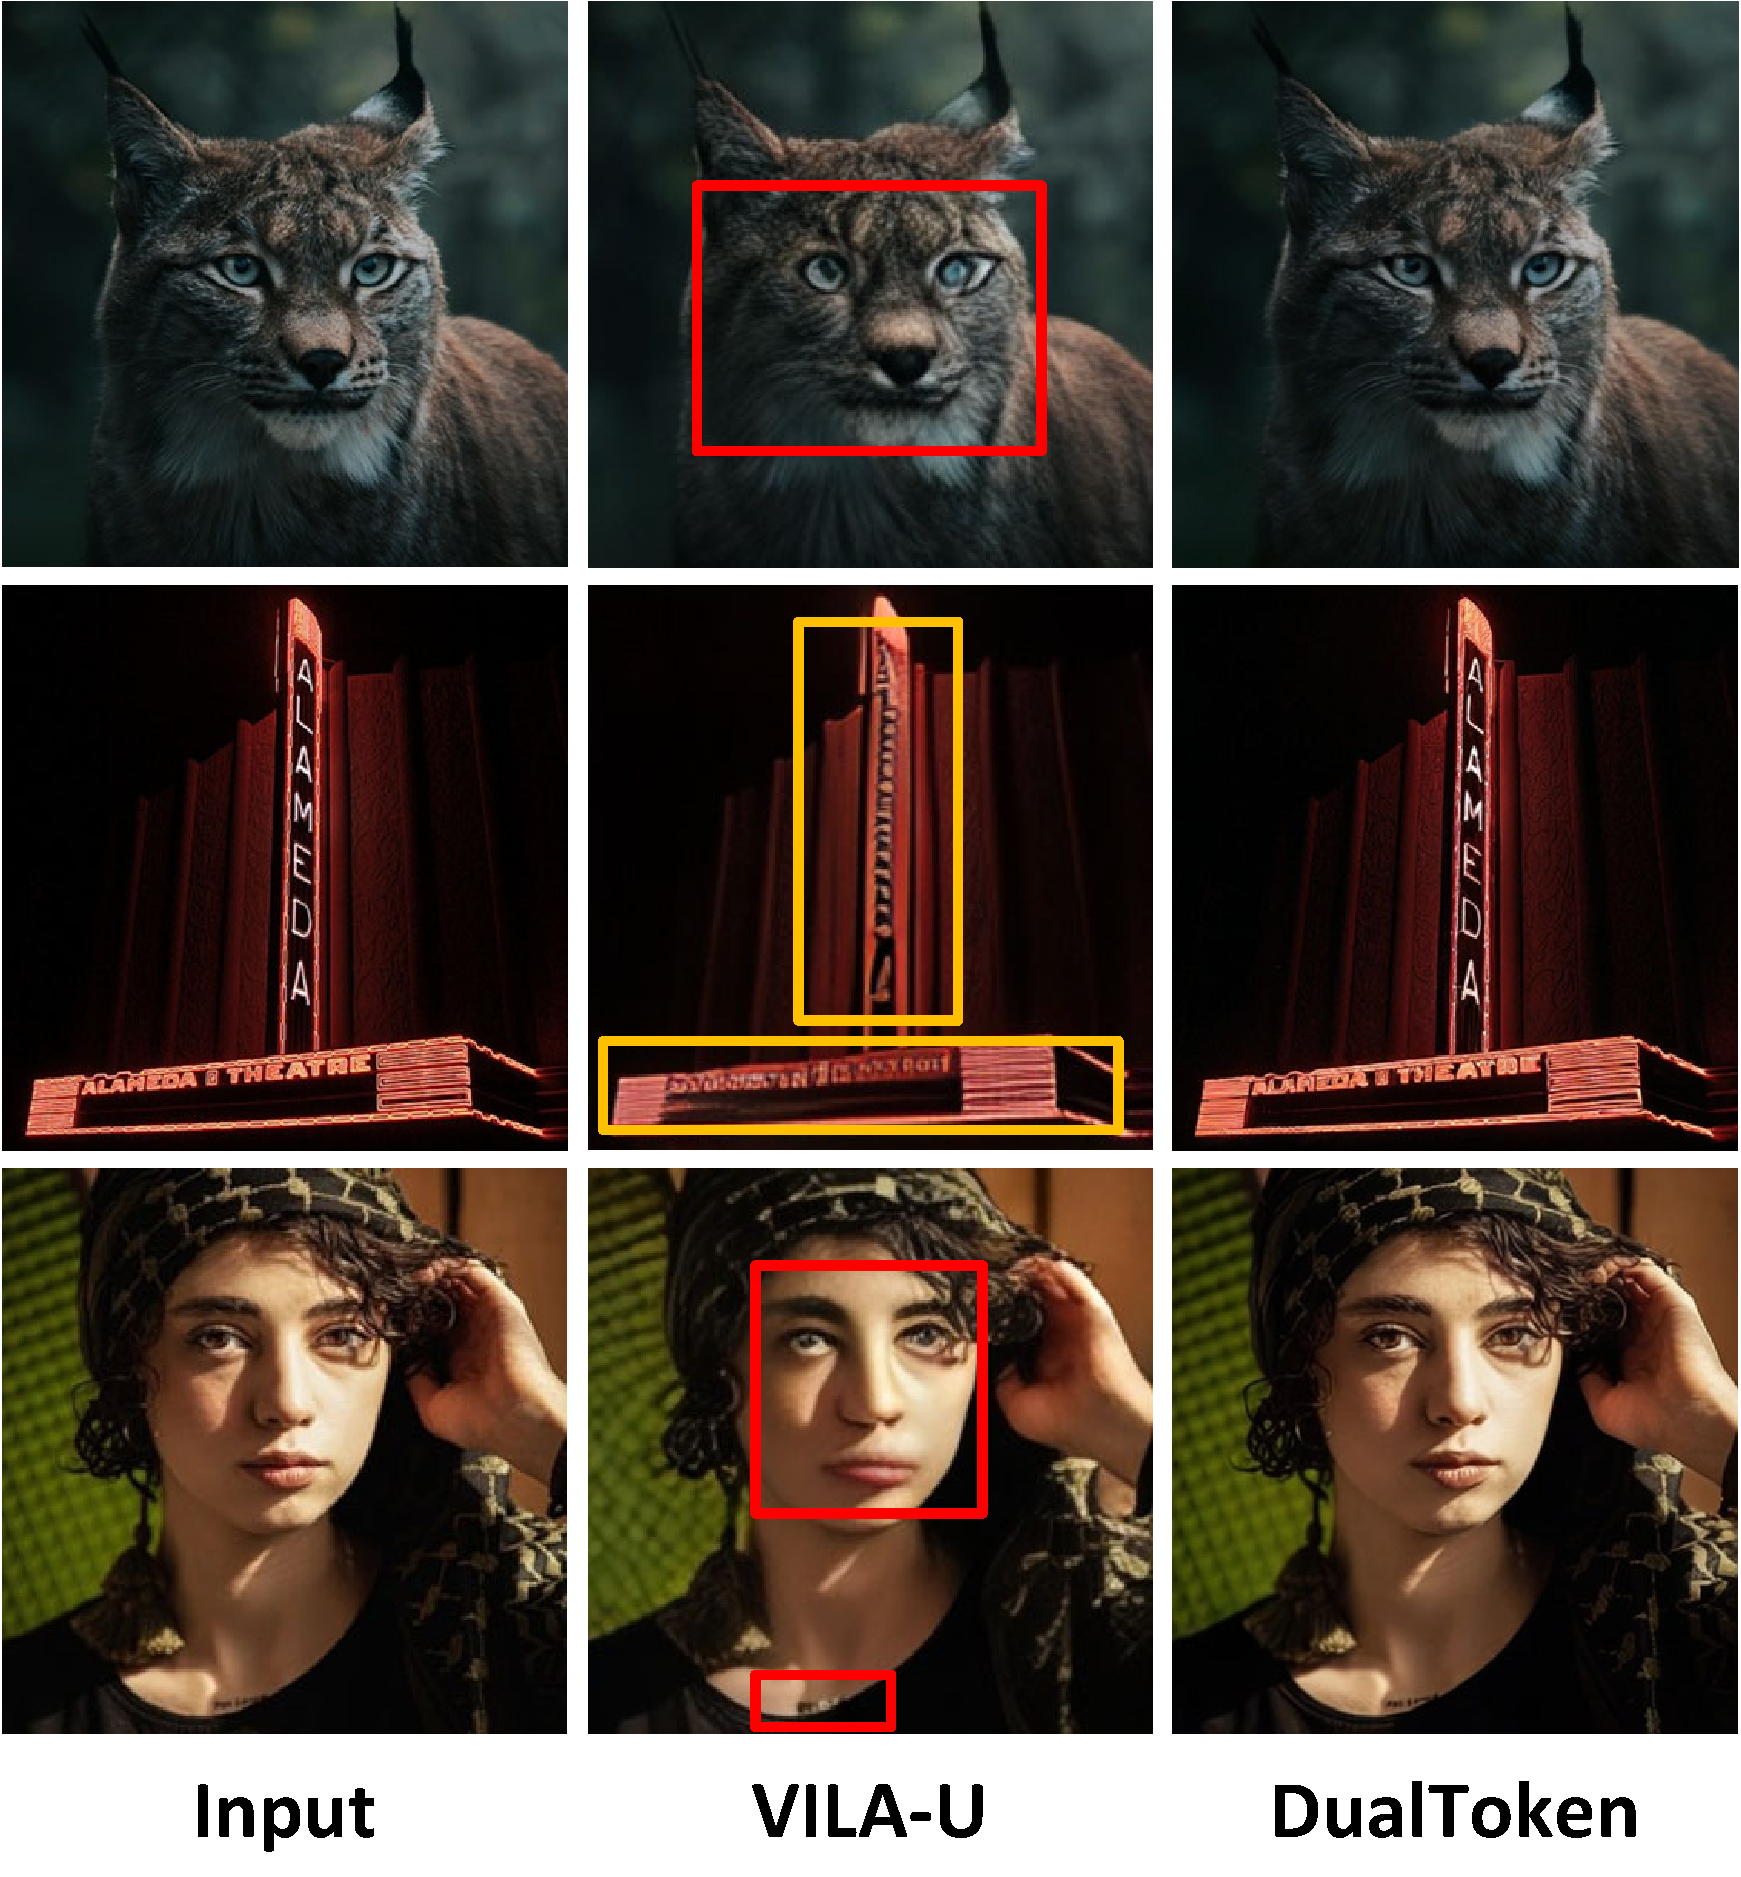
\includegraphics[height=5.2cm]{imgs/teaser.pdf}
%   \end{minipage}
%   \caption{
%     \textbf{Comparison with state-of-the-art vision encoders.} \textbf{(Left)} We compare zero-shot classification accuracy and reconstruction FID on ImageNet-1K(val) across baseline methods and \ours{}. \ours{} achieves results comparable to or surpassing both semantic-only and reconstruction-only methods in both tasks. \textbf{(Right)} Reconstruction results of VILA-U and \ours{}, our \ours{} significantly outperforms VILA-U, which suffers from severe distortion and blurriness.
%   }
%   \label{fig:Bubble}
% \end{figure}

\begin{figure}[ht]
  \centering
  \vspace{-0.2cm}
  \begin{minipage}[t]{0.435\textwidth}
  \centering
  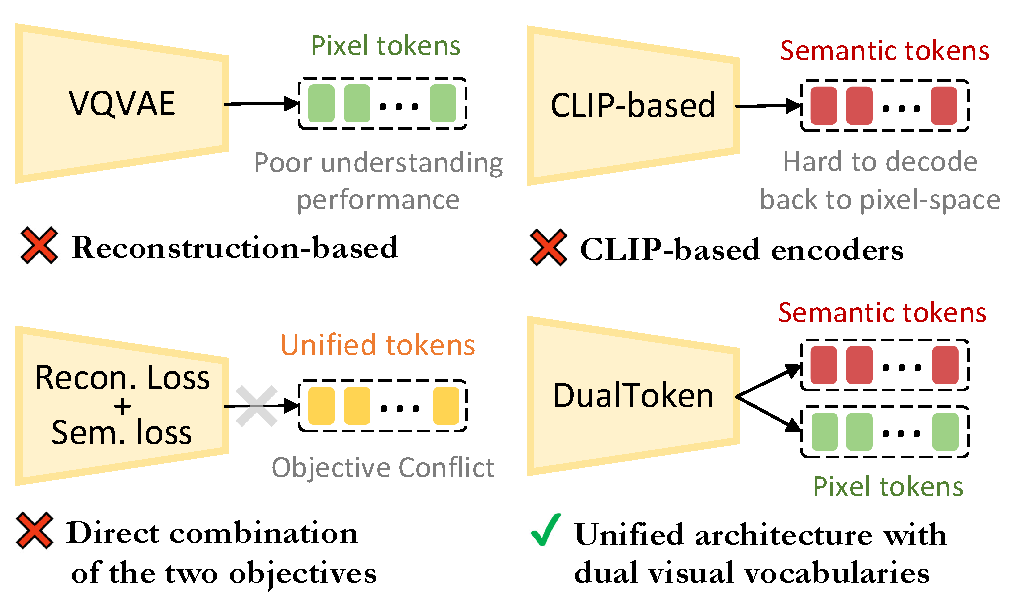
\includegraphics[height=3.5cm]{imgs/teaser_framework-v6.pdf}
  \end{minipage}
  \begin{minipage}[t]{0.303\textwidth}
  \centering
  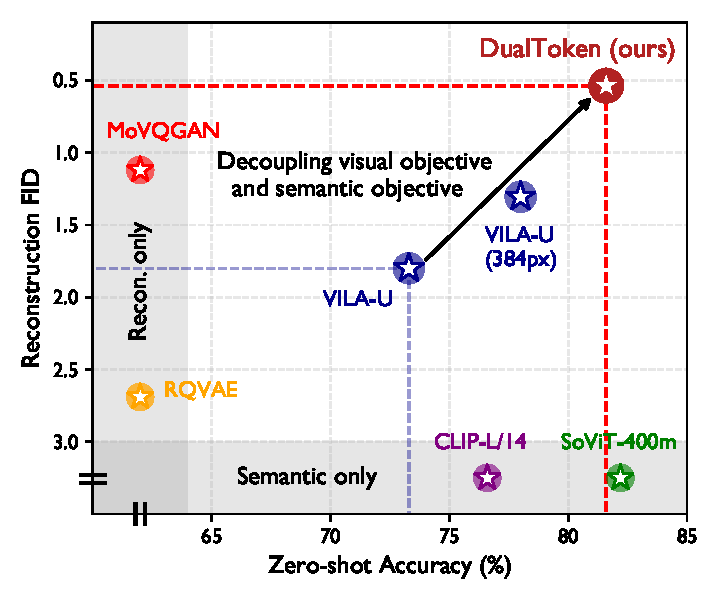
\includegraphics[height=3.5cm]{imgs/bubble.pdf}
  \end{minipage}
  \begin{minipage}[t]{0.250\textwidth}
  \centering
  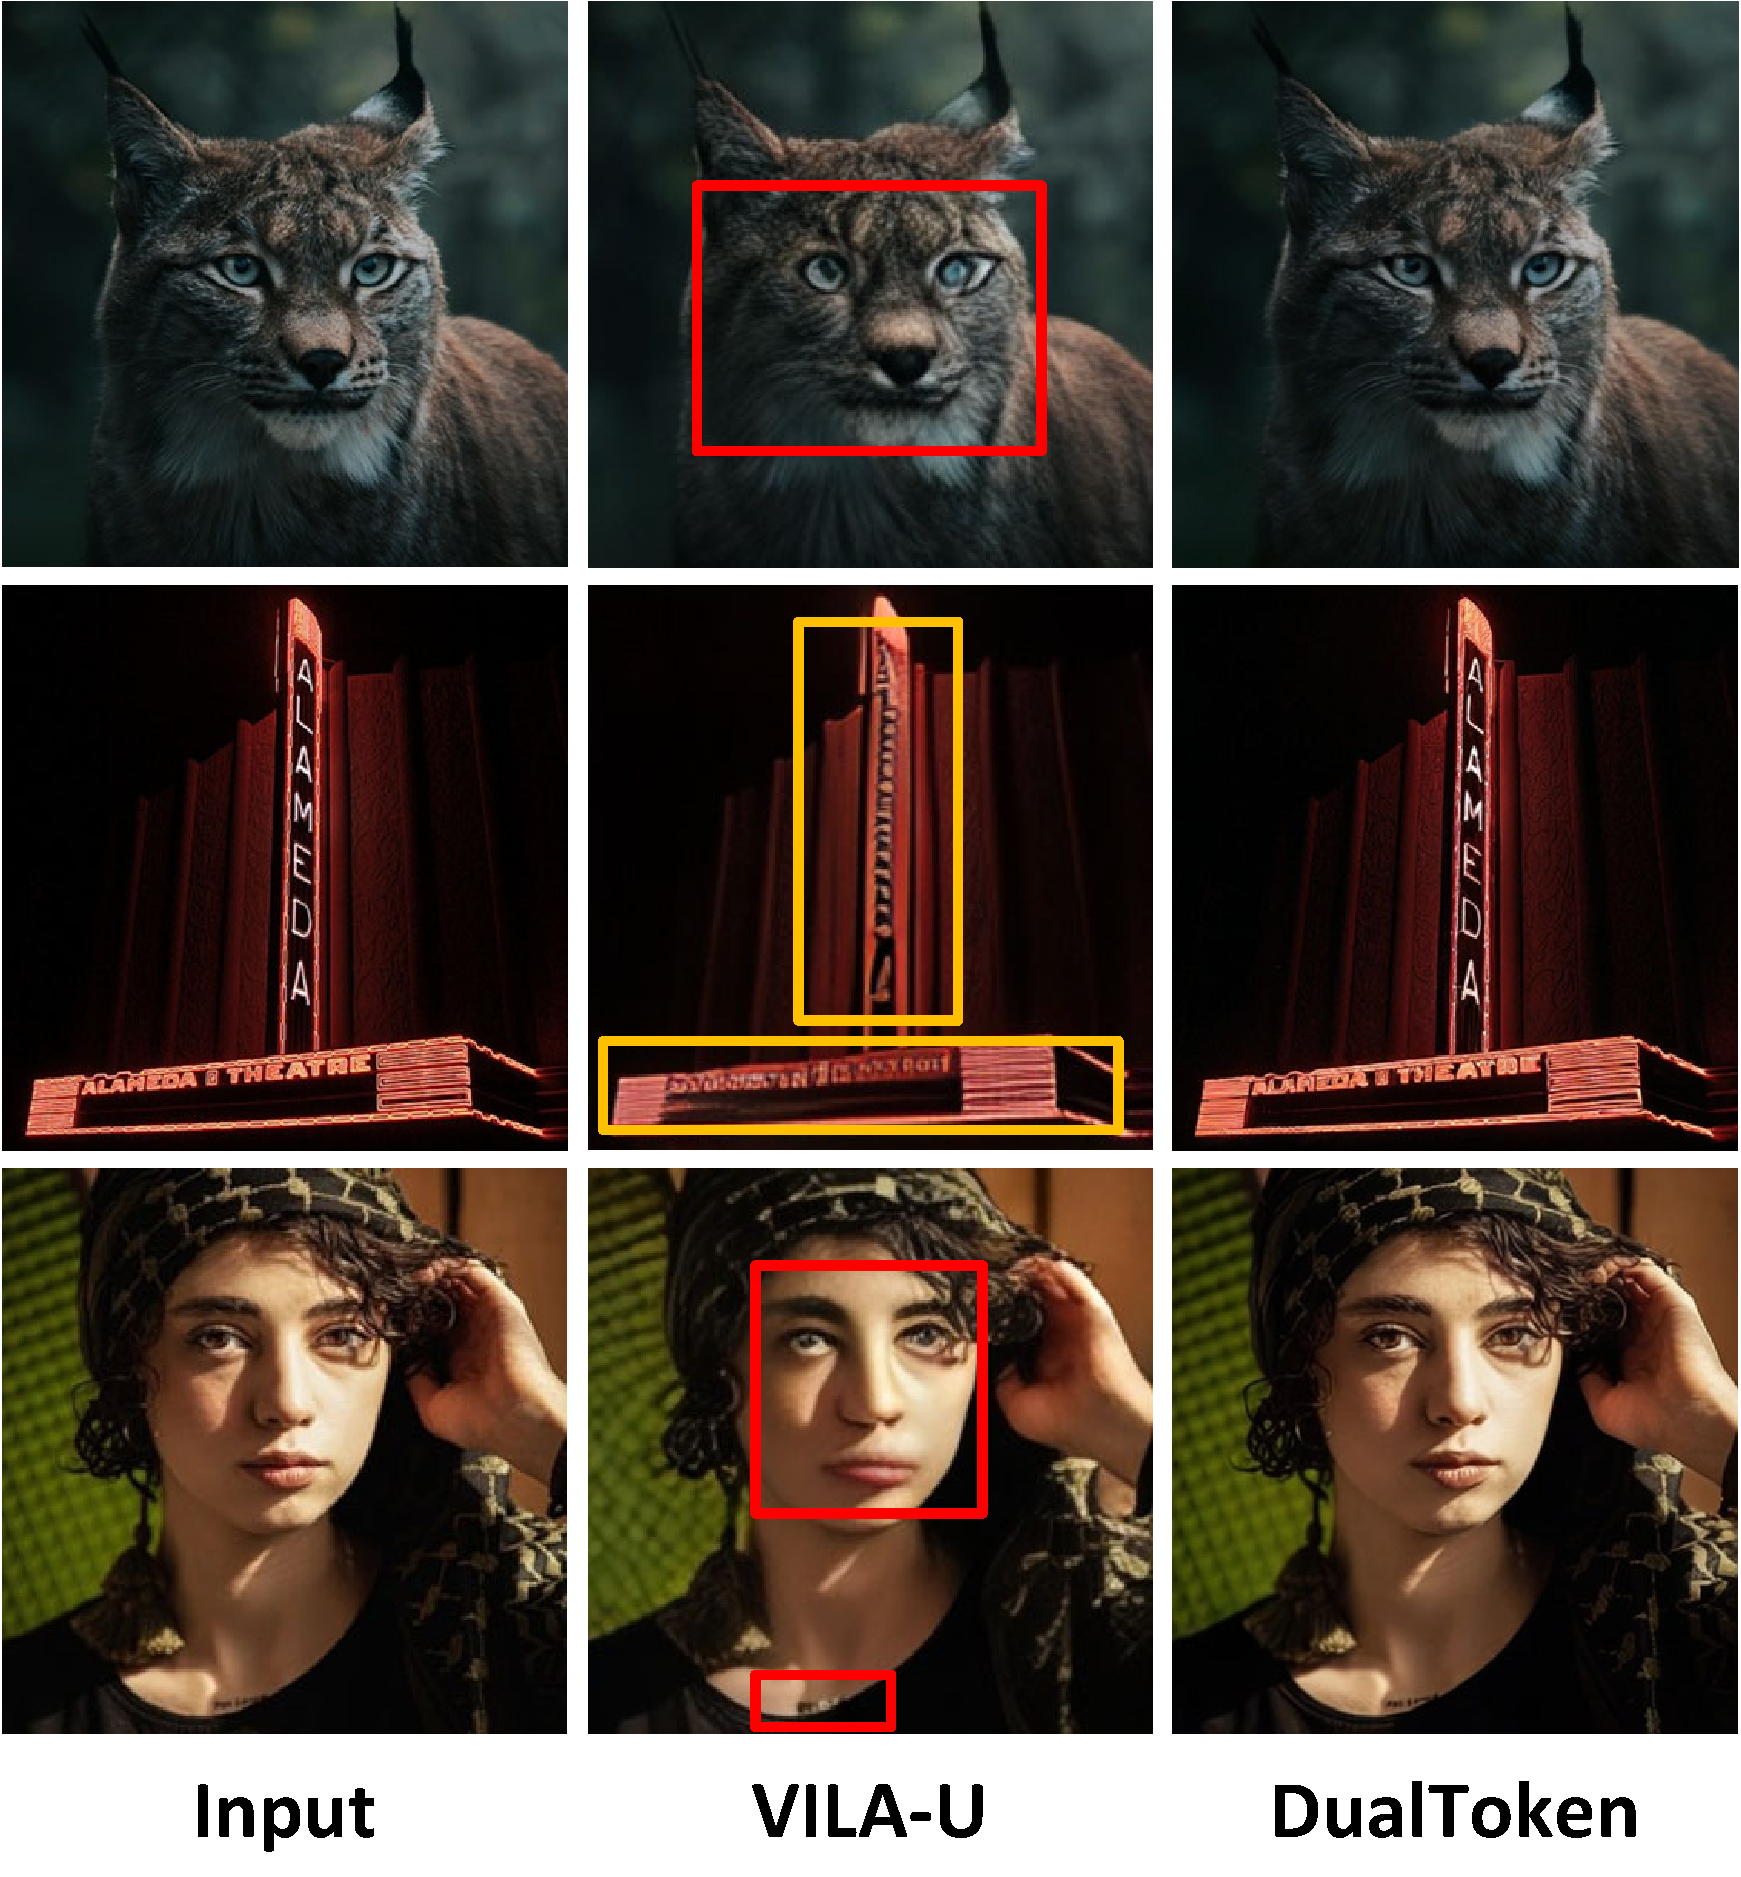
\includegraphics[height=3.5cm]{imgs/teaser.pdf}
  \end{minipage}
  
  \caption{
    \textbf{(Left)} Challenges faced by existing visual tokenizers. \textbf{(Middle)} We compare zero-shot classification accuracy and reconstruction FID on ImageNet-1K(val) across baseline methods and \ours{}. \ours{} achieves results comparable to or surpassing both semantic-only and reconstruction-only methods in both tasks. \textbf{(Right)} Reconstruction results of VILA-U and \ours{}, our \ours{} significantly outperforms VILA-U, which suffers from severe distortion and blurriness.
  }
  \label{fig:Bubble}
  % \vspace{-10pt}
  \vspace{-0.45cm}
\end{figure}
